\documentclass{scrreprt}
\usepackage{listings}
\usepackage{underscore}
\usepackage{graphicx}
\usepackage[bookmarks=true]{hyperref}
\usepackage[utf8]{inputenc}
\usepackage[german]{babel}
\hypersetup{
    bookmarks=false,    % show bookmarks bar?
    pdftitle={Software Requirement Specification},    % title
    pdfauthor={Fischer, Tobias \\
Libak, Miklós \\
Norkunas, Eva \\
Weinknecht, Lucas \\},                     % author
    pdfsubject={TeX and LaTeX},                        % subject of the document
    pdfkeywords={TeX, LaTeX, graphics, images}, % list of keywords
    colorlinks=true,       % false: boxed links; true: colored links
    linkcolor=blue,       % color of internal links
    citecolor=black,       % color of links to bibliography
    filecolor=black,        % color of file links
    urlcolor=purple,        % color of external links
    linktoc=page            % only page is linked
}%
\def\myversion{0.1 }
\date{}
%\title

\newcommand{\lstinlinejava}[1]{\lstinline[language=java]{#1}}
\newcommand{\lstj}[1]{\lstinlinejava{#1}}


\lstset{language=Java,
  showspaces=false,
  showtabs=false,
  breaklines=true,
  showstringspaces=false,
  breakatwhitespace=true,
  commentstyle=\color{pgreen},
  keywordstyle=\color{pblue},
  stringstyle=\color{pred},
  basicstyle=\ttfamily,
  moredelim=[il][\textcolor{pgrey}]{$$},
  moredelim=[is][\textcolor{pgrey}]{\%\%}{\%\%}
}


\hypersetup{
    colorlinks=true,
    linkcolor=blue,
    filecolor=magenta,      
    urlcolor=cyan,
}

\usepackage{color}

\definecolor{pblue}{rgb}{0.13,0.13,0.7}
\definecolor{pgreen}{rgb}{0,0.5,0}
\definecolor{pred}{rgb}{0.9,0,0}
\definecolor{pgrey}{rgb}{0.46,0.45,0.48}
\usepackage{hyperref}

\usepackage{enumitem,amssymb}
\newlist{todolist}{itemize}{2}
\setlist[todolist]{label=$\square$}
\usepackage{pifont}
\newcommand{\cmark}{\ding{51}}%
\newcommand{\xmark}{\ding{55}}%
\newcommand{\done}{\rlap{$\square$}{\raisebox{2pt}{\large\hspace{1pt}\cmark}}%
\hspace{-2.5pt}}
\newcommand{\wontfix}{\rlap{$\square$}{\large\hspace{1pt}\xmark}}


\begin{document}

\begin{flushright}
    \rule{16cm}{5pt}\vskip1cm
    \begin{bfseries}
        \Huge{SOFTWARE REQUIREMENTS\\ SPECIFICATION}\\
        \vspace{1.5cm}
        for\\
        \vspace{1.5cm}
        MELT Chess\\
        \vspace{1.5cm}
        \LARGE{Version \myversion}\\
        \vspace{1.5cm}
        \vspace{1.5cm}
        \today\\
    \end{bfseries}
\end{flushright}

\tableofcontents

\chapter{Einführung}

\section{Projektanforderungen}
Entwickelt werden soll ein Schach Programm, welches es ermöglicht gegeneinander als auch gegen eine künstliche Intelligenz Schach zu spielen. Das Spiel soll dafür sowohl über eine graphische als auch über eine konsolenbasierte Benutzerschnittstelle verfügen. Das Spiel soll in englischer Sprache umgesetzt werden. Die Entwicklung soll sich dabei in drei Iterationen gliedern. In diesem Dokument sind die Anforderungen an die erste Iteration dargelegt.

\section{Zielgruppe des Dokuments und weitere Resourcen}
Dieses Anforderungsdokument richtet sich zum einen an die beteiligten Entwickler und dient zur Orientierung ob die Funktionalität des Projekt gemäß den Anforderungen umgesetzt wird, und zum anderen an die Kontaktperson(en) des Moduls um die Planung des Projekts zu überprüfen.

Einen weiteren Überblick bieten die Storycards, welche im Gitlab des Projekts zu finden sind und in Form von Issues umgesetzt werden.

\chapter{Umfang des Projekts}
\section{Funktionale Anforderungen}
Zum Umfang gehört in der 1. Iteration des Projekts die Bereitstellung einer Textbasierten Konsolen-Schnittstelle in der es möglich ist Mensch-gegen-Mensch Spiele zu spielen. Dazu ist die Umsetzung des Pakets model nötig, in dem der Zustand des Bretts sowie die Schachregeln\footnote{Nach den Regeln des Weltschachverbands (FIDE) in der deutschen Übersetzung von 2018} implementiert werden.

In der 2. Iteration wird die geschaffene Basis durch eine 2D-GUI unter Verwendung des JavaFX Moduls erweitert und eine rudimentäre Schach KI im Modul engine erstellt.

In der 3. Iteration soll die Anwendung um Netzwerkfähigkeit mit der Anwendung der Gruppe 2 erweitert werden. Zusätzlich soll eine Auswahl von möglichen Erweiterungen umgesetzt werden, welche in Summe einen Aufwand von mindestens 10 Einheiten aufweisen müssen. Die Auswahl mit möglicher Punktzahl lauten:

\begin{itemize}
\item Verbesserte KI mithilfe Min-/Max-Suche mit $\alpha$/$\beta$-Pruning (5)
\item 3D-GUI (5)
\item Eindimensionales Schach (5)
\item Rückgängig-Machen von Zügen (3)
\item Speichern/Laden von Spielen (3)
\item Schachuhren (2)
\item Zweisprachigkeit (2)
\item Resizeable GUI (1)
\end{itemize}

\section{Nicht-funktionale Anforderungen}

\subsection{Codingstyle, Metriken, Testabdeckung}
Das Template verwendet die Plugins PMD und JaCoCo zur Generierung von Reports über Metriken, Codestyle und Testabdeckung.
Es wird eine Testabdeckung des gesamten Codes von 90\% Instruction Coverage erwartet, ausgenommen der GUI-Klassen.
Im Template wird ein PMD-Regelsatz eingebunden. Diese Regeln sind für den Code und die Testfälle einzuhalten.


\subsection{Überprüfungen}
Es soll mindestens alle zwei Wochen ein Treffen mit dem zugewiesenen Tutor stattfinden. Neben den Deadlines der drei Iterationen gibt es außerdem noch folgende Termine:

\begin{itemize}
\item 23.04.2021: Abgabe Anforderungsanalyse, Vorgehensplan, Prüfung erfolgreiche Einrichtung der Infrastruktur

\item 19.05.2021: Prüfung, ob auslieferbare Version vorliegt, die Anforderungen der ersten Iteration genügt mit automatisierten Tests und Theorie-Abfrage

\item 16.06.2021: Prüfung, ob auslieferbare Version vorliegt, die
Anforderungen der zweiten Iteration genügt mit Zwischenpräsentation

\item 14.07.2021: Endabgabe mit Abschlusspräsentation
\end{itemize}

\subsection{Abgabeformat}
An den Schlusstagen der Iterationen, inklusive Endabgabe, muss der zu überprüfende/bewertende Stand mittels Tags (it1,it2,...) im git-Repository gekennzeichnet werden.




\chapter{Vorgehensplan}
Der Vorgehensplan wurde durch Storycards im Issuetracker von gitlab realisiert. Für die Dauer des Praktikums können diese \href{https://projects.isp.uni-luebeck.de/melt-chess/melt-chess/-/issues}{hier}\footnote{https://projects.isp.uni-luebeck.de/melt-chess/melt-chess/-/issues} eingesehen werden. Im Folgenden befindet sich eine maschinell generierte Version aus dem csv Export von gitlab.

\section{Storycard Issues}



\subsection*{Schnittstelle Konsole}
id: \#3 Milestone: 1. Iteration\\

\begin{itemize}
\item[Priorisierung] A
\item[Storypoints] 5
\item[Risiko] high
\end{itemize}

Der Benutzer hat die Möglichkeit das Schachspiel gegen einen anderen Benutzer zu spielen. Dazu werden die Züge in der Konsole eingegeben.

\textbf{Abgeschlossen wenn}
\begin{todolist}
    \item[\done]  Die Benutzereingabe wird korrekt geparsed (Tests für ``parseUserMoveInput`` bestanden)
  \item[\done]  Gameloop ist etabliert (User Input einlesen, Schachbrettposition ausgeben, ...)
  \item[\done]  Ausgabe der geschlagenen Figuren auf den Befehl ``beaten``
  \item[\done]  Ausgabe wenn ein Spieler im Schach steht
  \item[\done]  Die Anforderungen an die Ausgabe bei gesetztem ``
  \item[\done]  Fehleingabe wird mit ``!Invalid move`` quittiert
  \item[\done]  Gültige Eingabe wird mit ``!<Eingabe>``quittiert
  \item[\done]  Ein ungültiger Zug wird mit ``!Move not allowed``quittiert
  \item[\done]  Schachbrett wird nach jedem Zug geprintet
  \item[\done]  Matt oder Unentschieden wird angezeigt und dadurch wird das Spiel beendet
  \item[\done]  Es gibt einen Befehl, um das Spiel zu beenden
  \item[\done]  Nach einer falschen Eingabe wird auf eine neue Eingabe gewartet

\end{todolist}


\subsection*{Erstellen der Models}
id: \#4 Milestone: 1. Iteration\\

\begin{itemize}
\item[Priorisierung] A
\item[Storypoints] 31
\item[Risiko] high
\end{itemize}

Erstellen der Klassen im Paket \lstj{models} welche von den anderen Paketen \lstj{cli}, \lstj{engine} und \lstj{gui} benutzt werden

\textbf{Abgeschlossen wenn}
\begin{todolist}
    \item[\done]  Alle blockierenden Storycards sind abgeschlossen

\end{todolist}


\subsection*{Erstellen Board Klasse}
id: \#5 Milestone: 1. Iteration\\

\begin{itemize}
\item[Priorisierung] B
\item[Storypoints] 2
\item[Risiko] low
\end{itemize}

Die \lstj{Board} Klasse im Paket \lstj{model} kapselt eine Position auf dem Brett, sowie die Information welcher Spieler am Zug ist. Die Position wird dabei als Array mit 64 Integerwerten zwischen 0 und 23 kodiert.

\textbf{Abgeschlossen wenn}
\begin{todolist}
    \item[\done]  Die Klasse repräsentiert eine Position auf dem Brett
  \item[\done]  Ein neues Objekt kann durch übergeben eines FEN
  \item[\done]  Ein neues Objekt kann durch die ``makeMove`` Methode aus einem bestehenden Objekt erzeugt werden
  \item[\done]  Die Methoden ``getPiecePositionsFor`` und ``getPieceAt`` bestehen alle mithilfe von FEN

\end{todolist}


\subsection*{Erstellen Move Klasse}
id: \#6 Milestone: 1. Iteration\\

\begin{itemize}
\item[Priorisierung] B
\item[Storypoints] 1
\item[Risiko] low
\end{itemize}

Die \lstj{Move} Klasse im Paket \lstj{model} soll einen Container für einen Spielzug verwirklichen. Sie merkt sich dazu von und zu welchem Feld der Zug gemacht wird, sowie eine Flag die besondere Umstände des Zugs (Rochade, Figurentausch, ...) beschreibt.

\textbf{Abgeschlossen wenn}
\begin{todolist}
    \item[\done]  Die Informationen zu einem Zug werden erfolgreich kodiert
  \item[\done]  Die toString Methode gibt eine String repräsentation des Zuges gemäß den Anforderungen des Konsolen Clients zurück

\end{todolist}


\subsection*{Erstellen der MoveGenerator Klasse}
id: \#7 Milestone: 1. Iteration\\

\begin{itemize}
\item[Priorisierung] C
\item[Storypoints] 13
\item[Risiko] high
\end{itemize}

Die \lstj{MoveGenerator} Klasse im Paket \lstj{model} soll mögliche Züge zu einer gegebenen Position unter berücksichtigung der Schachregeln generieren. Die werden sowohl von der GUI zum hervorheben der möglichen Felder beim bewegen einer Figur, als auch von der Engine bei der Suche nach dem nächsten Zug verwendet.

\textbf{Abgeschlossen wenn}
\begin{todolist}
    \item[\done]  Der Generator kann die verschiedenen Laufrichtungen zu den unterschiedlichen Schachfiguren berechnen
  \item[\done]  Die ``generate`` Methoden bestehen sinnvolle Tests (Siehe die Flags in der Klasse ``Move``: werden auch diese Züge gefunden?)

\end{todolist}


\subsection*{Erstellen der Piece Klasse}
id: \#8 Milestone: 1. Iteration\\

\begin{itemize}
\item[Priorisierung] B
\item[Storypoints] 2
\item[Risiko] low
\end{itemize}

Die Klasse \lstj{Piece}im Paket \lstj{model} soll die geplanten statischen Methoden zur Extraktion der kodierten Informationen zur Verfügung stellen. Typ und Farbe einer Schachfigur wird dabei als Integer zwischen 0 und 23 kodiert.

\textbf{Abgeschlossen wenn}
\begin{todolist}
    \item[\done]  Die statischen Methoden zur Rückgabe der in einem Integer Wert codierten Informationen bestehen alle Tests.
  \item[\done]  Die toString Methode gibt die vorher festgelegten Symbole korrekt wieder

\end{todolist}


\subsection*{Erstellen der 2D GUI}
id: \#9 Milestone: 2. Iteration\\

\begin{itemize}
\item[Priorisierung] E
\item[Storypoints] 34
\item[Risiko] high
\end{itemize}

Zum planen GUI für die Folgenden Schritte weitere Issues anlegen und mit \#9 verlinken: Design, Architektur, Implementierung

\textbf{Abgeschlossen wenn}
\begin{todolist}
    \item[\done]  Klare Vorstellung wie die GUI aussehen soll (Design)
  \item[\done]  Die Architektur wurde geplant
  \item[\done]  Die GUI wurde implementiert

\end{todolist}


\subsection*{Erstellen der Engine}
id: \#10 Milestone: 2. Iteration\\

\begin{itemize}
\item[Priorisierung] A
\item[Storypoints] 13
\item[Risiko] high
\end{itemize}

Erstellen der Klasse \lstj{Engine} im Paket \lstj{engine}. Die Engine berechnet zu einer \lstj{Board}-Instanz einen neuen Zug.

\textbf{Abgeschlossen wenn}
\begin{todolist}
    \item[\done]  Die Engine ist in der Lage ein paar einfache ausgewählte Schachprobleme zu lösen
  \item[\done]  Die Engine kann sinnvolle nächste Züge für ein PVPC Spiel generieren

\end{todolist}


\subsection*{Erstellen MoveValidator Klasse}
id: \#11 Milestone: 1. Iteration\\

\begin{itemize}
\item[Priorisierung] D
\item[Storypoints] 8
\item[Risiko] high
\end{itemize}

Der \lstj{MoveValidator} soll die vom \lstj{MoveGenerator} berechneten Züge auf gültigkeit überprüfen. Da die erlaubten Bewegungsrichtungen bereits in \lstj{MoveGenerator} korrekt implementiert sind, müssen hauptsächlich die Sonderregeln die zu schach des Königs führen beachtet werden. 

\textbf{Abgeschlossen wenn}
\begin{todolist}
    \item[\done]  Der König kann nicht in schach bewegt werden
  \item[\done]  Gefesselte eigene Figuren können den König nicht in Schach setzen
  \item[\done]  Ist "im schach" implementiert, wurde das generieren von Rochadezügen in ``MoveGenerator`` verhindert. Edit: Die Züge werden zwar generiert, aber vom ``MoveValidator`` abgelehnt.

\end{todolist}


\subsection*{Erstellen der Game Klasse}
id: \#12 Milestone: 1. Iteration\\

\begin{itemize}
\item[Priorisierung] E
\item[Storypoints] 3
\item[Risiko] low
\end{itemize}

Die \lstj{Game} Klasse soll den Gesamtzustand einer Partie kapseln, aber hauptsächlich für die beiden GUI Module relevant sein.

\textbf{Abgeschlossen wenn}
\begin{todolist}
    \item[\done]  Funktion für "neues Spiel starten"
  \item[\done]  Verwaltet alle nötigen Objekte einer Partie und bietet ein einfaches Interface für die GUI Module
  \item[\done]  Erkennt Schachmatt und Patt (\#13 )

\end{todolist}


\subsection*{Schachmatt und Patt}
id: \#13 Milestone: 1. Iteration\\

\begin{itemize}
\item[Priorisierung] E
\item[Storypoints] 2
\item[Risiko] low
\end{itemize}

Es müssen die Fälle Patt (ein Spieler hat keine möglichen Züge) und Schachmatt (ein Spieler hat keine möglichen Züge und steht im Schach) implementiert werden

\textbf{Abgeschlossen wenn}
\begin{todolist}
    \item[\done]  Partie kann in Patt enden
  \item[\done]  Partie kann durch schachmatt gewonnen/verloren werden

\end{todolist}


\subsection*{Testen von model und cli}
id: \#14 Milestone: 1. Iteration\\

\begin{itemize}
\item[Priorisierung] A
\item[Storypoints] 8
\item[Risiko] high
\end{itemize}

Testen der Konsolenschnittstelle und damit auch des \lstj{model} Pakets mittels der bereitgestellten checker App.

\textbf{Abgeschlossen wenn}
\begin{todolist}
    \item[\done]  checker App läuft und kann MELT Chess ausführen
  \item[\done]  Bugs und nicht bestandene Tests sind behoben

\end{todolist}


\subsection*{Erstellen MenuController}
id: \#15 Milestone: 2. Iteration\\

\begin{itemize}
\item[Priorisierung] C
\item[Storypoints] 13
\item[Risiko] high
\end{itemize}

Der `MenuController` interpretiert die Aktionen des Benutzers, die dieser über die [`MenuView`](\#16) ausführt.

\textbf{Abgeschlossen wenn}
\begin{todolist}
    \item[\done]  Der Benutzer kann einen von drei Spielmodi wählen: "Game against AI / Spiel gegen KI", "Game against second player / Spiel gegen zweiten Spieler" oder "Network game / Netzwerkspiel". Der gewählte Modus muss sich grafisch abheben.
  \item[\done]  Der Benutzer kann eine von zwei Farben der Spielfiguren wählen: weiß oder schwarz. Die gewählte Farbe muss sich grafisch abheben.
  \item[\done]  Die Taste "Start game / Spiel starten" startet das Spiel gegen die KI, gegen den zweiten Spieler oder startet das Netzwerkspiel, je nachdem, was der Benutzer ausgewählt hat
  \item[\done]  Die Taste "Settings / Einstellungen" öffnet das Einstellungsmenü

\end{todolist}


\subsection*{Erstellen MenuView}
id: \#16 Milestone: 2. Iteration\\

\begin{itemize}
\item[Priorisierung] A
\item[Storypoints] 8
\item[Risiko] high
\end{itemize}

Zeigt dem Benutzer das Hauptmenü an.

\textbf{Abgeschlossen wenn}
\begin{todolist}
    \item[\done]  Enthält drei Tasten zur Auswahl des Spielmodus: "Game against AI / Spiel gegen KI", "Game against second player / Spiel gegen zweiten Spieler" und "Network game / Netzwerkspiel". Die ausgewählte Taste muss sich grafisch abheben.`handleRadioButtonAIOnAction``handleRadioButtonPVPOnAction``handleRadioButtonNetOnAction`
  \item[\done]  Enthält zwei Tasten zur Auswahl der Farbe der Spielfiguren: weiß und schwarz. Die ausgewählte Taste muss sich grafisch abheben.`handleRadioButtonColorBlackOnAction``handleRadioButtonColorWhiteOnAction`
  \item[\done]  Enthält Spielstarttaste "Start game / Spiel starten"`handleButtonStartOnAction`
  \item[\done]  Enthält eine Taste "Settings / Einstellungen" zum Öffnen der Einstellungen`handleButtonSettingsOnAction`

\end{todolist}


\subsection*{Erstellen SettingsView}
id: \#17 Milestone: 2. Iteration\\

\begin{itemize}
\item[Priorisierung] A
\item[Storypoints] 13
\item[Risiko] high
\end{itemize}

Zeigt dem Benutzer das Einstellungen an.

\textbf{Abgeschlossen wenn}
\begin{todolist}
    \item[\done]  Enthält eine Taste "Save / Speichern" zum Speichern der Einstellungen.`handleButtonSaveOnAction`
  \item[\done]  Enthält Taste "Cancel / Abbrechen" zum Verlassen der Einstellungen.`handleButtonCancelOnAction`
  \item[\done]  Enthält eine Label mit dem Text "Interface language / Interfacesprache".
  \item[\done]  Enthält zwei Radio Buttons mit möglichen Sprachen.`handleRadioButtonEnOnAction``handleRadioButtonDeOnAction`
  \item[\done]  Enthält ein Kontrollkästchen mit dem Text "Rotate the chessboard after each move / Das Schachbrett nach jedem Zug drehen".`handleCheckboxFlipBoardOnAction`
  \item[\done]  Enthält ein Kontrollkästchen mit dem Text "One
  \item[\done]  Enthält ein Kontrollkästchen mit dem Text "Show that the player is in check / Zeigen, dass der Spieler in Schach ist".`handleCheckboxShowInCheckOnAction`
  \item[\done]  Enthält ein Kontrollkästchen mit dem Text "Show possible moves when selecting a character / Mögliche Züge bei Auswahl einer Figur anzeigen".`handleCheckboxShowPossibleMovesOnAction`

\end{todolist}


\subsection*{Erstellen SettingsController}
id: \#18 Milestone: 2. Iteration\\

\begin{itemize}
\item[Priorisierung] C
\item[Storypoints] 13
\item[Risiko] high
\end{itemize}

Der `SettingsController` interpretiert die Aktionen des Benutzers, die dieser über die [`SettingsView`](\#17) ausführt.

\textbf{Abgeschlossen wenn}
\begin{todolist}
    \item[\done]  Der Benutzer kann die Sprache über das Auswahlmenü ändern.
  \item[\done]  Mit der Taste "Save / Speichern" kann der Benutzer die geänderten Einstellungen speichern.
  \item[\done]  Mit der Taste "Cancel / Abbrechen" kann der Benutzer die geänderten Einstellungen verwerfen und das Einstellungsfenster verlassen.
  \item[\done]  Der Benutzer kann das Kontrollkästchen verwenden, um "Rotate the chessboard after each move / Das Schachbrett nach jedem Zug drehen" zu aktivieren oder zu deaktivieren.
  \item[\done]  Der Benutzer kann das Kontrollkästchen verwenden, um "One
  \item[\done]  Der Benutzer kann das Kontrollkästchen verwenden, um "Show that the player is in check / Zeigen, dass der Spieler in Schach ist" zu aktivieren oder zu deaktivieren.
  \item[\done]  Der Benutzer kann das Kontrollkästchen verwenden, um "Show possible moves when selecting a character / Mögliche Züge bei Auswahl einer Figur anzeigen" zu aktivieren oder zu deaktivieren.

\end{todolist}


\subsection*{Erstellen Settings Klasse}
id: \#19 Milestone: 2. Iteration\\

\begin{itemize}
\item[Priorisierung] 
\item[Storypoints] 
\item[Risiko] S
\end{itemize}

Speichert den Status der aktuellen Einstellungen und stellt sie zur Abfrage bereit.

\textbf{Abgeschlossen wenn}
\begin{todolist}
    \item[\done]  Die Klasse besitzt alle nötigen Felder für die verschiedenen Einstellungsmöglichkeiten
  \item  Die Klasse kann serialsiert werden

\end{todolist}


\subsection*{Erstellen TextManager Klasse}
id: \#20 Milestone: 2. Iteration\\

\begin{itemize}
\item[Priorisierung] B
\item[Storypoints] 8
\item[Risiko] low
\end{itemize}

Steuert die Ausgabe des gewünschten Sprachpakets in Abhängigkeit von der aktuellen Sprache

\textbf{Abgeschlossen wenn}
\begin{todolist}
    \item[\done]  Andere Klassen können durch den 'TextManager' die Beschriftungen von Labels ändern lassen

\end{todolist}


\subsection*{Erstellen NetworkConnectView}
id: \#21 Milestone: 2. Iteration\\

\begin{itemize}
\item[Priorisierung] E
\item[Storypoints] 8
\item[Risiko] low
\end{itemize}

Die `NetworkConnectView` gibt dem Benutzer die Möglichkeit, die Daten für die Netzwerkverbindung einzugeben.

\textbf{Abgeschlossen wenn}
\begin{todolist}
    \item[\done]  Es gibt das Textfeld `textfieldIPAddress`, in dem die IP
  \item[\done]  Es gibt das Textfeld `textfieldPort`, in dem das entsprechende Port eingegeben werden kann. Dieses Textfeld ist mit dem Label `lblPort` "Port" versehen.
  \item[\done]  Es gibt das Label `lblConnectionFail` "Connection Error, check IP
  \item[\done]  Es gibt den Button `handleConnectSaveOnAction` "Connect"/"Verbinden".
  \item[\done]  Es gibt den Button `handleButtonCancelOnAction` "Cancel"/"Abbrechen".

\end{todolist}


\subsection*{Erstellen NetworkConnectController}
id: \#22 Milestone: 2. Iteration\\

\begin{itemize}
\item[Priorisierung] 
\item[Storypoints] 
\item[Risiko] D
\end{itemize}

Der `NetworkConnectController` interpretiert die Aktionen des Benutzers, die dieser über die `NetworkConnectView` ausführt.

\textbf{Abgeschlossen wenn}
\begin{todolist}
    \item  Bei Klick auf `btnConnect` wird das `lblConnectionFail` auf "unsichtbar" geändert und ein Verbindungsaufbau entsprechend der Nutzereingabe versucht.
  \item  Schlägt die Verbindung fehl, wird die Sichtbarkeit von `lblConnectionFail` auf "sichtbar" geändert.
  \item  Gelingt die Verbindung, so wird die `GameView` als aktuelle `Scene` gesetzt.
  \item[\done]  Bei einem Klick auf `btnCancel` wird die `MainMenueView` als aktuelle `scene` gesetzt.

\end{todolist}


\subsection*{Erstellen GameView}
id: \#23 Milestone: 2. Iteration\\

\begin{itemize}
\item[Priorisierung] A
\item[Storypoints] 21
\item[Risiko] high
\end{itemize}

Die `GameView` ist die View, in der der Nutzer das eigentliche Spiel spielen kann, hier kann er Züge eingeben und das Spielfeld sehen.

\textbf{Abgeschlossen wenn}
\begin{todolist}
    \item[\done]  Es gibt den Button `handleButtonSettingsOnAction` "Settings"/"Einstellungen".
  \item[\done]  Es gibt den Button `handleButtonResetOnAction` "Reset"/"Zurücksetzen".
  \item[\done]  Es gibt den Button `handleButtonSurrenderOnAction` "Surrender"/"Aufgeben".
  \item[\done]  Es gibt den Button `handleButtonMenueOnAction` "Main Menue"/"Hauptmenü".
  \item[\done]  Es gibt das Label `lblHistory` darin werden die ausgeführten Züge aufgelistet. Dieses Label sollte scrollbar sein.
  \item[\done]  Es gibt ein Canvas `canvasField`, das die Musterung des Schachfeldes zeigt.
  \item[\done]  Es gibt die Möglichkeit, die Grafik der aktuellen Aufstellung der Figuren auf dem `canvasField` zu zeigen.
  \item[\done]  Es gibt das Label `lblCheckMessage`, das im Initialzustand unsichtbar ist. Hier werden Informationen wie "Check!"/"Schach!" oder "Check Mate"/"Schachmatt" angezeigt.
  \item[\done]  Es gibt das Label `lblInfo`, das anzeigen soll, welche Farbe am Zug ist. Das muss nicht zwingend ein Label sein, sonder könnte auch als Farbfeld realisiert werden.

\end{todolist}


\subsection*{Erstellen GameController}
id: \#24 Milestone: 2. Iteration\\

\begin{itemize}
\item[Priorisierung] C
\item[Storypoints] 13
\item[Risiko] high
\end{itemize}

Der `GameController` interpretiert die Aktionen des Benutzers, die dieser über die [GameView](\#23) ausführt.

\textbf{Abgeschlossen wenn}
\begin{todolist}
    \item[\done]  Der Button `btnSettings` setzt die `SettingsView` als aktuelle `Scene`.
  \item[\done]  Der Inhalt des Labels `lblHistory` wird nach jedem Zug entsprechend aktualisiert.
  \item[\done]  Der Button `btnMainMenue` setzt die `MainMenueView` als aktuelle `Scene`.
  \item[\done]  Der Button `btnReset` setzt das Spiel zurück, also ein neues Spiel im aktuellen Modus wird gestartet. Das sollte wahrscheinlich aber im NetworkGame nicht möglich sein.
  \item[\done]  Das Label `lblInfo` wird im Fall von Schach (wenn das in den Einstellungen so konfiguriert ist) mit dem Text "Check!"/"Schach!" auf sichtbar gesetzt und beim nächsten Zug aber wieder auf unsichtbar gesetzt.
  \item[\done]  Das Label `lblCheckMessage` wird im Fall von Schachmatt mit dem Text "Check Mate, game over!"/"Schachmatt, Spiel vorbei!" auf sichtbar gesetzt.
  \item[\done]  Das Label `lblInfo` zeigt immer, welche Farbe am Zug ist. Das muss nicht zwingend ein Label sein, sonder könnte auch als Farbfeld realisiert werden.
  \item[\done]  Der `GameViewController` kann sich von der Klasse `BoardGraphics` die grafische Umsetzung des aktuellen Aufstellung holen und diese in dem `canvasField` über der Musterung des Schachfeldes anzeigen. Das muss nach jedem Zug passieren.
  \item[\done]  Der `GameViewController` achtet darauf ob und wo in das Canvas `canvasField` geklickt wird. Wenn dort was passiert, verarbeitet er das Event entsprechend.

\end{todolist}


\subsection*{Erstellen GraphicsManager}
id: \#25 Milestone: 2. Iteration\\

\begin{itemize}
\item[Priorisierung] B
\item[Storypoints] 8
\item[Risiko] high
\end{itemize}

Die `GraphicsManger`-Klasse Verwaltet die grundsätzliche Verwendung von allen verwendeten Grafiken. Nur auf diesem Weg soll ein Zugriff auf unsere Grafiken möglich sein.

\textbf{Abgeschlossen wenn}
\begin{todolist}
    \item[\done]  Andere Klassen können bestimmte Grafiken anfordern.

\end{todolist}


\subsection*{Erstellen BoardController}
id: \#26 Milestone: 2. Iteration\\

\begin{itemize}
\item[Priorisierung] C
\item[Storypoints] 21
\item[Risiko] high
\end{itemize}

Die `BoardController`-Klasse kontrolliert, was passiert, wenn auf das Schachfbrett geklickt wird. Sie benutzt dabei `BoardModel`, um relevante Informationen zu erhalten und kann auch Informationen in `BoardModel` verändern.

\textbf{Abgeschlossen wenn}
\begin{todolist}
    \item[\done]  Aus einem übergebenen Cursor
  \item[\done]  Speichert im `BoardModel`, welches genaue Feld angeklickt wurde.
  \item[\done]  Kann das `BoardModel` fragen, ob bereits ein genaues Feld angeklickt wurde.
  \item[\done]  Kann das `SettignsModel` fragen, ob es erlaubt ist, ein bestimmtes Feld anzuklicken.
  \item[\done]  Kann aus einem `Board` die Positionen (Koordinaten) für Graphiken bestimmen und das Ergebnis im `BoardModel` speichern. Das gilt für die Grafiken von den Figuren, für die geschlagenen Figuren und für die Grafiken der Markierungen.

\end{todolist}


\subsection*{Erstellen BoardModel}
id: \#27 Milestone: 2. Iteration\\

\begin{itemize}
\item[Priorisierung] B
\item[Storypoints] 8
\item[Risiko] high
\end{itemize}

Hier werden Informationen über das gerade sichtbare Schachbrett gespeichert. Dazu gehören die Positionen von den Grafiken, welche Figur gerade ausgewählt ist etc.

\textbf{Abgeschlossen wenn}
\begin{todolist}
    \item[\done]  speichert ob eine Figur ausgewählt ist.
  \item[\done]  speichert welche Figur ausgewählt ist.
  \item[\done]  speichert eine Liste der geschlagenen Figuren als `ImageView`

\end{todolist}




\chapter{Anhang}
\section{Tabellarische Anforderungsanalyse}
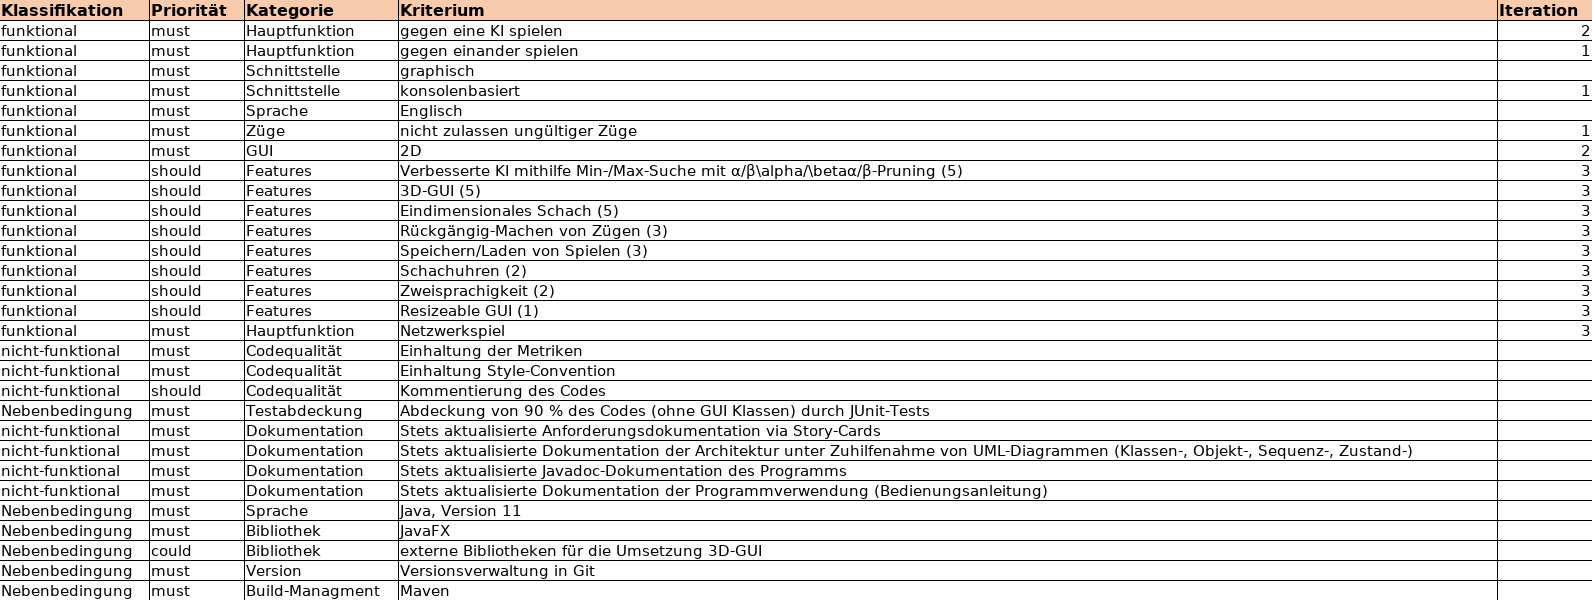
\includegraphics{resources/anforderungsanalyse_tabelle.png}
\end{document}
